This Section describes first what data storage is and which typologies of storage exist. Thus, this project's data storage layer, \gls{HopsFS}, is presented, starting from its evolution from \gls{HDFS}, going into the details about its tools, and ending with possible alternatives, the cloud object storages.

\subsection{Block storage vs. File storage vs. Object storage}
\label{subsec:block_vs_file_vs_object}

Data can be stored and organized in physical storages, such as \glspl{HDD} or \glspl{SSD}. The three main type of data storage are (1)~Block storage, (2)~File storage, and (3)~Object storage briefly compared in Table \ref{tab:short_storage_comparison}. Each typology is describe in the following paragraphs, and their pros and cons are summarized in Table \ref{tab:long_storage_comparison}. This Subsection is a re-elaboration of three articles from major cloud providers (Amazon, Google, and IBM) \cite{BlockVsFile, HowObjectVs, ObjectVsFile2021} according to the author's understanding.

\begin{table}[!ht]
    \begin{center}
      \caption[Data storage features comparison]{Data storage features comparison. Table inspired by major cloud providers articles \cite{BlockVsFile,HowObjectVs,ObjectVsFile2021}.}
      \label{tab:short_storage_comparison}
      \begin{tabular}{cccc}
        \toprule
        \textbf{Characteristics} & \textbf{Block Storage} & \textbf{File Storage} & \textbf{Object Storage}\\
        \midrule
        Performance & High & High & Low\\
        Scalability & Low & Low & High\\
        Cost & High & High & Low\\
        \bottomrule
      \end{tabular}
    \end{center}
\end{table}

\subsubsection*{Block Storage}

Block storage is a data storage method that divides data into discrete blocks of fixed size, each assigned a unique identifier. These blocks are stored independently on a storage system, such as a \gls{SAN} or within a cloud environment. 

This decentralized approach offers several key advantages. Firstly, it enables high performance with fast read/write speeds and low latency, crucial for demanding applications like databases and virtual machine environments. Secondly, block storage provides direct, low-level access to storage volumes, similar to physical disks, granting users and applications granular control over data organization and management. This flexibility allows for a wide range of use cases, including powering virtual machine environments, supporting high-performance databases, and enabling efficient file sharing.

While offering significant benefits, block storage also presents certain limitations. It typically requires specialized hardware and infrastructure, potentially leading to higher costs compared to other storage options. Furthermore, while it offers a degree of scalability, expanding beyond certain limits can become complex and costly. Despite these considerations, block storage remains a vital technology for modern IT environments, enabling high performance, flexibility, and agility in data management.

\subsubsection*{File Storage}

File storage is a hierarchical data organization method that stores data in files, which are organized into folders within a structure of directories and subdirectories. Files are characterized by extensions (e.g., ".txt", ".png", ".csv"), defining how the data is organized and accessed. This system simplifies locating and retrieving individual files when their exact paths are known, making it intuitive and user-friendly.

This structure is particularly beneficial for managing structured data and is widely used in \gls{PC} and \gls{NAS} devices. It enables centralized file sharing on  \gls{LAN} and supports common file-level protocols, ensuring compatibility across Windows and Linux systems. Storing data on a separate NAS device or in the cloud also enhances data protection and disaster recovery, with options to replicate data across multiple geographic locations for added security.

However, as the volume of files grows, scaling becomes challenging. Locating files in a large hierarchy can be time-consuming, and scaling often requires investing in additional or higher-capacity hardware. Cloud-based file storage services mitigate these challenges by offering scalable, off-site storage managed by service providers. These services eliminate hardware maintenance costs and provide flexible, subscription-based models that adapt to varying storage and performance needs.

File storage remains popular for applications requiring simplicity and centralized access, such as file sharing, personal storage, and cloud-based platforms like Dropbox and Google Drive. While other storage solutions may be better suited for managing massive datasets or unstructured data, file storage's accessibility, affordability, and ease of use ensure its ongoing relevance.

\subsubsection*{Object Storage}

Object storage is a flat data storage method that organizes data into self-contained objects, each containing metadata that describes attributes like size, creation date, and unique identifiers. This metadata not only defines the data but also enables efficient querying and retrieval of large datasets. This makes object storage particularly well-suited for managing unstructured data, such as videos, images, and other media files that do not fit neatly into traditional hierarchical systems.

The flat structure of object storage eliminates complex hierarchies like folders and directories, simplifying organization and improving scalability. This structure allows object storage systems to replicate data across multiple regions, enhancing accessibility and fault tolerance in case of hardware failures. As a result, users benefit from faster data access in different parts of the world and robust disaster recovery options.

However, object storage has limitations. Objects are immutable, meaning they cannot be directly altered once created. Any changes require the creation of a new object. Additionally, object storage does not support transactional operations, as it lacks mechanisms like file locking, making it unsuitable for applications requiring frequent updates or real-time data changes. It also has slower writing performance compared to file or block storage solutions.

Overall, object storage is an excellent choice for use cases requiring high scalability, such as social networks, video streaming platforms, and cloud-based services. Its flat structure and metadata-driven design are ideal for managing large, static datasets. However, other storage options are preferred when high performance is required for frequently changing files or when transactional consistency is critical.

\begin{table}[h!]
    \centering
    \caption[Data storage pros and cons comparison]{Data storage pros and cons comparison. Table inspired by major cloud providers articles \cite{BlockVsFile,HowObjectVs,ObjectVsFile2021}.}
    \label{tab:long_storage_comparison}
    \begin{tabular}{|p{1.8cm}|p{4.8cm}|p{5.3cm}|}
        \hline
        \textbf{Storage Typology} & \textbf{Pros} & \textbf{Cons} \\
        \hline
        Block & 
        \begin{tabular}[t]{@{}l@{}}
            High performance \\ 
            High reliability \\ 
            Easy updates
        \end{tabular} & 
        \begin{tabular}[t]{@{}l@{}}
            Lacks metadata \\ 
            Not easily searchable \\ 
            High cost
        \end{tabular} \\
        \hline
        File & 
        \begin{tabular}[t]{@{}l@{}}
            Easy on small-scale \\ 
            User-friendly \\ 
            User-manageable \\ 
            File-level locking
        \end{tabular} & 
        \begin{tabular}[t]{@{}l@{}}
            Inefficient on unstructured data \\ 
            Limited scalability
        \end{tabular} \\
        \hline
        Object & 
        \begin{tabular}[t]{@{}l@{}}
            Ideal on unstructured data \\ 
            Cost-effective \\ 
            Highly scalable \\ 
            Efficient advanced retrieval \\ 
        \end{tabular} & 
        \begin{tabular}[t]{@{}l@{}}
            No file-level locking \\ 
            Low performance \\ 
            No data updates
        \end{tabular} \\
        \hline
    \end{tabular}
\end{table}

\subsection{\glsfmtlong{HDFS}}
% Restart from
\gls{HDFS}, a distributed file system~\footnote{\gls{HDFS} official guide available at \url{https://hadoop.apache.org/docs/r1.2.1/hdfs_user_guide.html}}, is designed to store and process massive datasets efficiently. It leverages a cluster of commodity hardware, allowing for cost-effective scalability and high availability. Unlike traditional file systems, \gls{HDFS} prioritizes high-throughput data access, making it well-suited for applications that process large volumes of data (higher than 100 GB), such as log analysis, data warehousing, and machine learning \cite{kalakarunReviewHadoopHDFS2013}.

At the core of \gls{HDFS} lies a master-slave architecture. A single Namenode acts as the central control point, managing the file system namespace, tracking file metadata, and controlling client access to files. Multiple Datanodes serve as worker nodes, each responsible for storing and managing a portion of the data within the cluster. \gls{HDFS} divides files into large blocks, which are then replicated across multiple Datanodes to ensure data redundancy and fault tolerance. This distributed storage approach enhances data availability and minimizes the risk of data loss due to hardware failures. Figure \ref{fig:hdfs_schema} presents a simplified visual representation of the Namenode read/write operations and Datanode orchestrating operations in \gls{HDFS}.

The Namenode maintains a comprehensive record of the file system namespace, including file locations, block mappings, and access permissions. This metadata is crucial for efficient data retrieval and processing. By strategically placing data replicas across different nodes, \gls{HDFS} minimizes data movement, optimizing performance and reducing network congestion. This aligns with the core principle that "moving computation is cheaper than moving data". \gls{HDFS} is designed for applications that primarily require write-once-read-many access patterns. This design choice simplifies data management and optimizes performance for batch processing tasks, where data is typically written once and then read multiple times for analysis or processing.

Furthermore, \gls{HDFS} relaxes some of the strict requirements defined by POSIX, such as low-latency access, to prioritize high-throughput data transfer. This allows \gls{HDFS} to efficiently handle large-scale data processing tasks, making it a cornerstone of many big data applications.

\begin{figure}[!ht]
    \begin{center}
      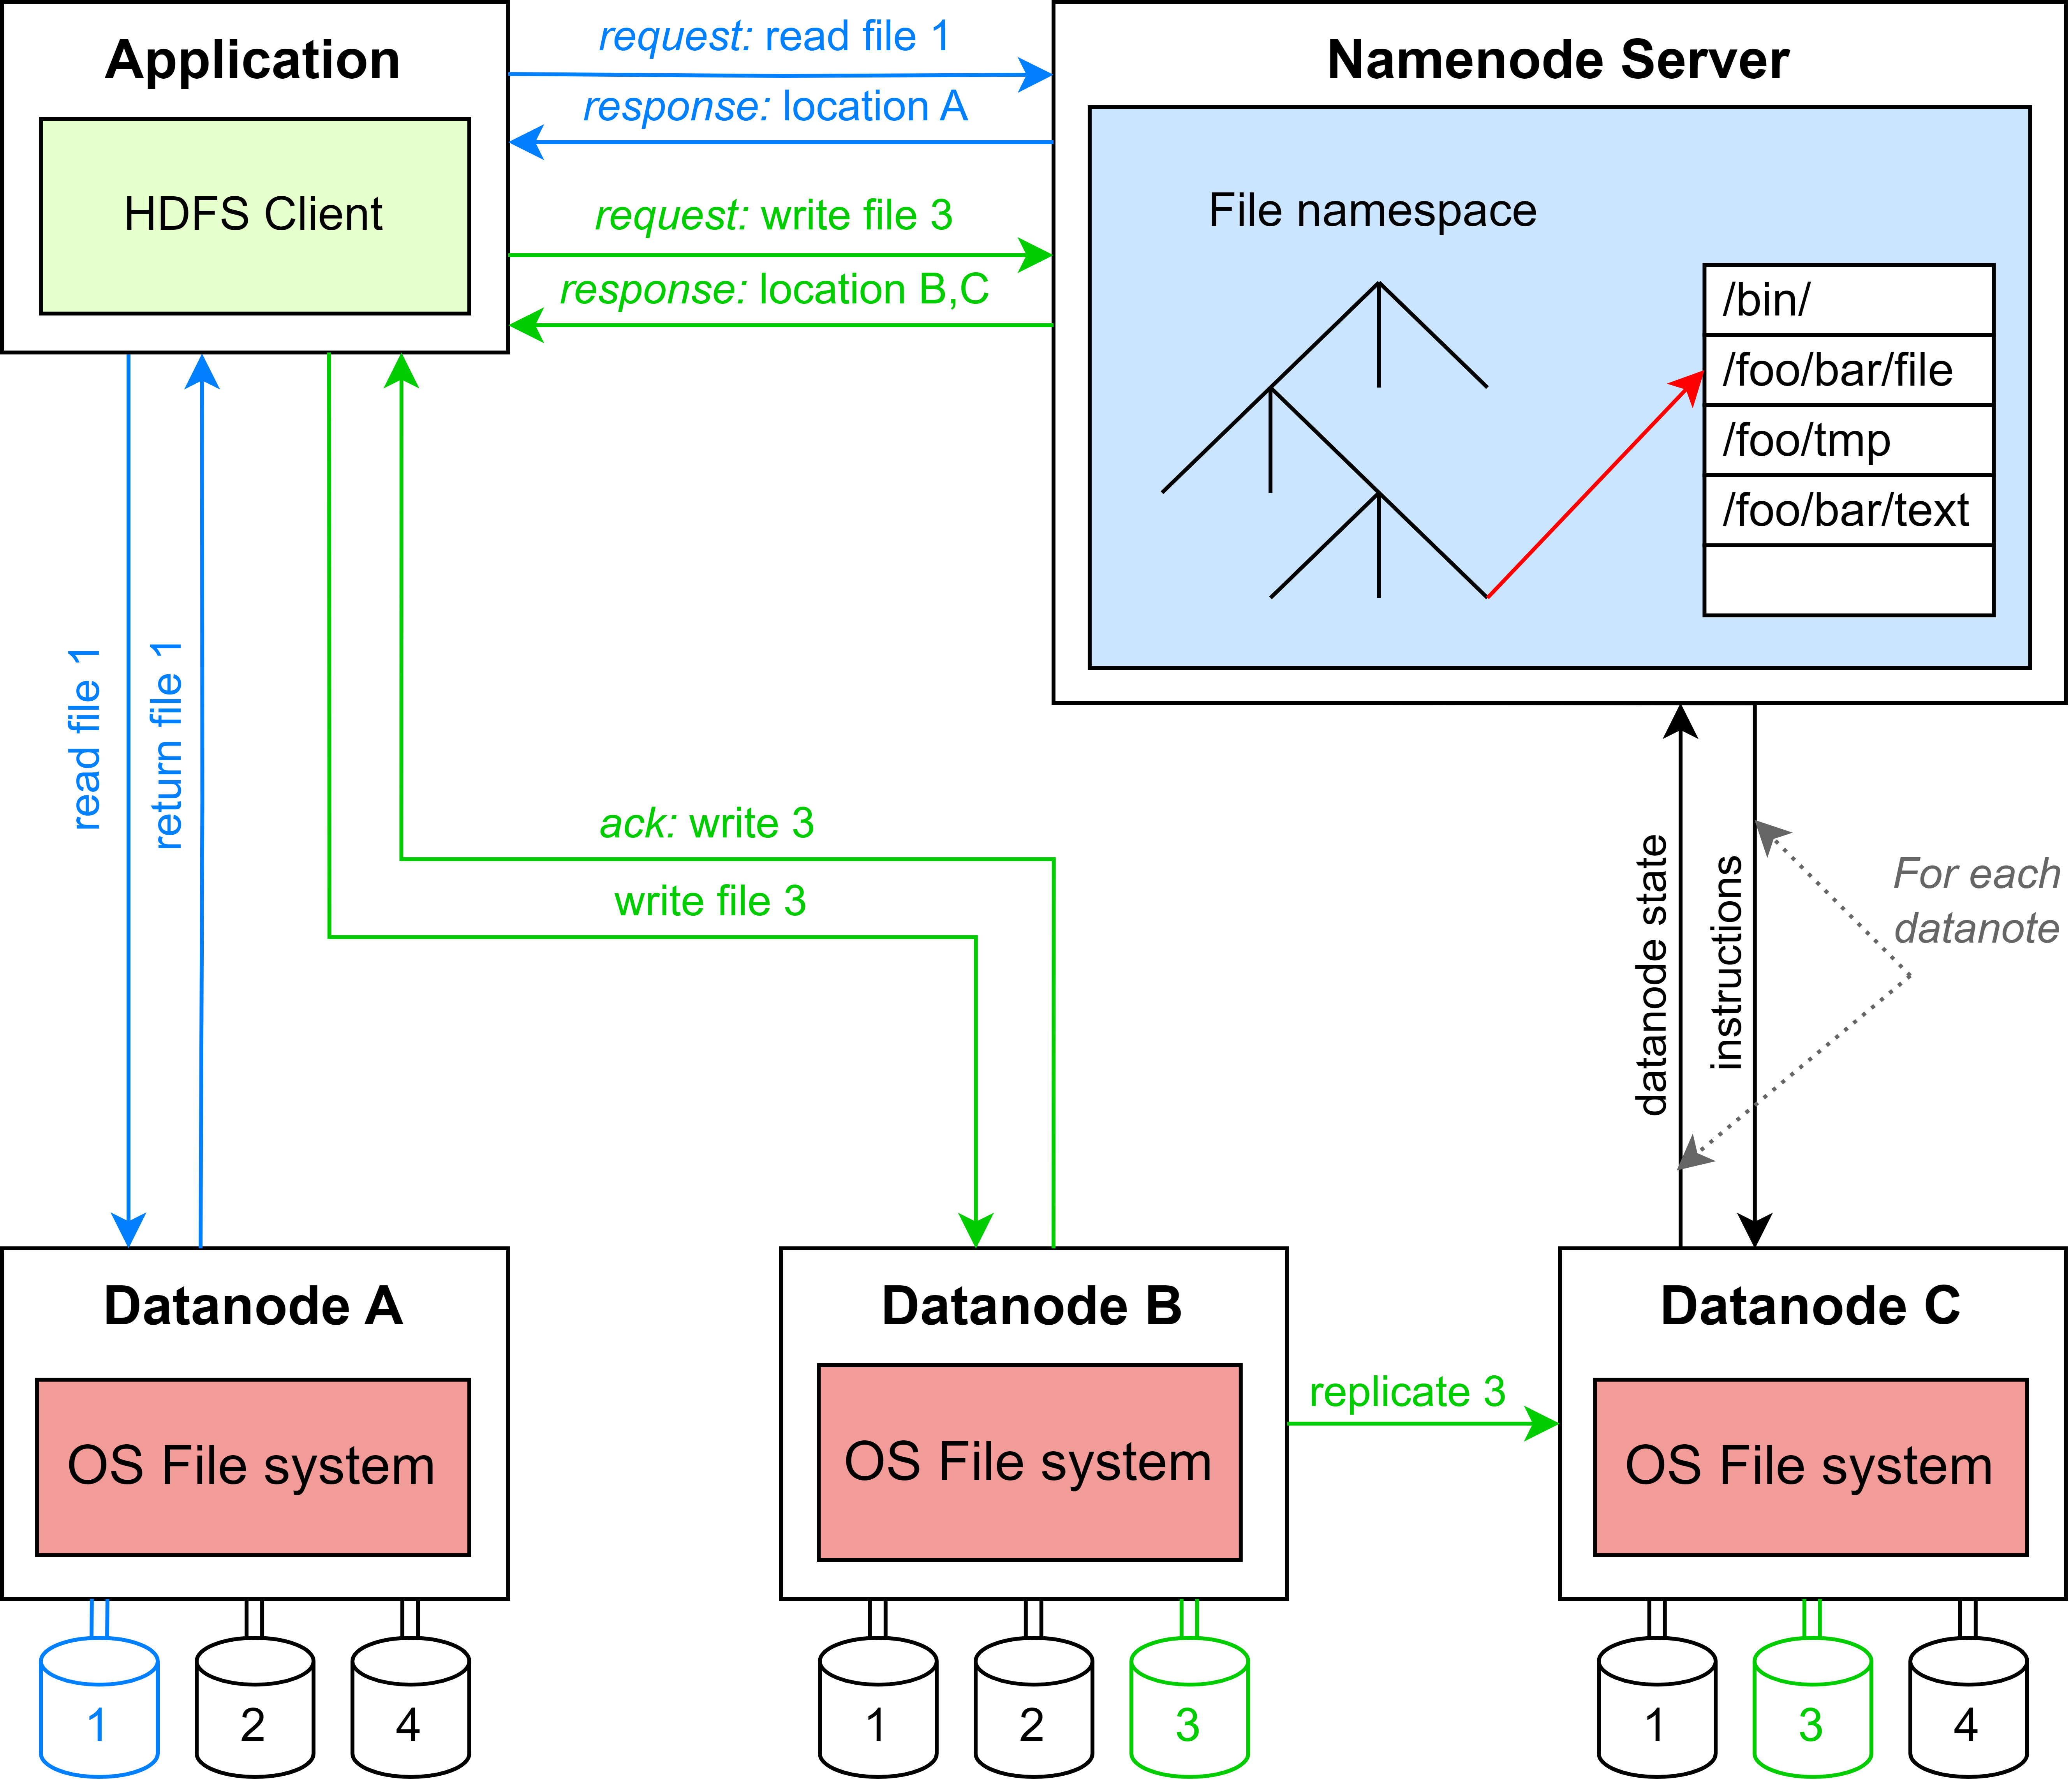
\includegraphics[width=\textwidth]{figures/2-background_and_related_work/hdfs_schema.png}
    \end{center}
    \caption[Hadoop Distributed File System architecture]{\glsentryfull{HDFS} architecture displaying in different colors basic operations: read (blue), write (green) and Namenode-Datanodes management messages (black). Note: for representation simplicity, files are not segmented into blocks and a single Namenode-Datanode message exchange is pictured. Diagram inspired by the Data-intensive Computing lectures at KTH by Prof. A. H. Payberah. Course website available at \url{https://www.kth.se/student/kurser/kurs/ID2221?l=en}.}
    \label{fig:hdfs_schema}
\end{figure}

\subsection{\glsfmtshort{HopsFS}}

\gls{HopsFS}, introduced at the 15th USENIX Conference in 2017 \cite{niaziHopsFSScalingHierarchical2017}, represents a significant evolution of \gls{HDFS}. \gls{HopsFS} addresses the critical scalability and metadata management limitations inherent to its predecessor, decentralizing metadata management by leveraging RonDB~\footnote{Details available at \url{https://www.rondb.com}}, a distributed NewSQL database, which allows metadata to be stored and managed across multiple Namenodes. This architecture supports Namenode replication and dynamic scaling, significantly enhancing throughput and operational efficiency.

\gls{HopsFS} encapsulates file system operations as distributed transactions, using advanced NewSQL features such as partition pruning and write-ahead caching. These techniques enable faster metadata retrieval and scalable operations, as seen in experiments where \gls{HopsFS} outperformed \gls{HDFS} by 16 to 37 times in throughput for real-world workloads \cite{10.1145/3626246.3653389}. Despite its scalability and performance advantages, \gls{HopsFS} remains backward-compatible with \gls{HDFS}, serving as a drop-in replacement. While \gls{HDFS} is widely adopted as a cornerstone of big data applications, \gls{HopsFS} provides a forward-looking solution for environments where metadata scalability and performance are critical. Both systems demonstrate the strengths of distributed file systems in managing massive datasets, but \gls{HopsFS} builds on the foundation of \gls{HDFS} by addressing its limitations and pushing the boundaries of what distributed file systems can achieve.

\subsection{Cloud object stores, an alternative}
The advent of cloud computing has revolutionized data storage, with object storage emerging as a dominant paradigm \cite{wuCloudStorageInfrastructure2010}. Pioneered by \gls{AWS} with its S3 service in 2006, cloud object storage services have rapidly proliferated, offered by major providers like \gls{GCS} and Microsoft Azure. This widespread adoption stems from the inherent advantages of cloud-based solutions, particularly their scalability and cost-effiency, as explained in \ref{subsec:block_vs_file_vs_object}. Cloud object storage empowers users to dynamically scale their storage capacity on-demand, paying only for the resources consumed. This pay-as-you-go model eliminates the need for significant upfront investments in hardware and infrastructure, significantly reducing operational costs. Furthermore, cloud providers leverage economies of scale to unparalleled levels of availability and scalability that are difficult to achieve for most organizations.

\gls{HDFS}, initially released in 2006, evolved alongside the rise of cloud object storage. While \gls{HDFS} has been widely adopted for on-premise deployments, the increasing popularity of cloud services has shifted the landscape. Cloud object storage solutions like \gls{AWS} S3, \gls{GCS}, and Azure Blob Storage have gained significant traction, with applications prioritizing support for these platforms due to their widespread adoption. While \gls{HDFS} and its advancements, such as \gls{HopsFS}, still have their place in specific use cases, the convenience and scalability offered by cloud object storage services have made them the preferred choice for many organizations. However, in the latest year, hybrid solution have been created, to extend cloud object storage with typical file-based system advantages, such has \gls{HopsFS}--S3 \cite{ismailHopsFSS3ExtendingObject2020}.